\documentclass[11p]{article}
% Packages
\usepackage{amsmath}
\usepackage{graphicx}
\usepackage{fancyheadings}
\usepackage[swedish]{babel}
\usepackage[
    backend=biber,
    style=authoryear-ibid,
    sorting=ynt
]{biblatex}
\usepackage[utf8]{inputenc}
\usepackage[T1]{fontenc}
%Källor
\addbibresource{references.bib}
\graphicspath{ {./images/} }

% Lite variabler
\def\email{endo.axelsson@ga.ntig.se}
\def\foottitle{PMmall}
\def\name{Endo Axelsson}

\title{PMmall \\ \small Gymnasiearbete}
\author{\name}
\date{\today}

\begin{document}

% fixar sidfot
\lfoot{\footnotesize{\name \\ \email}}
\rfoot{\footnotesize{\today}}
\lhead{\sc\footnotesize\foottitle}
\rhead{\nouppercase{\sc\footnotesize\leftmark}}
\pagestyle{fancy}
\renewcommand{\headrulewidth}{0.2pt}
\renewcommand{\footrulewidth}{0.2pt}

% i Sverige har vi normalt inget indrag vid nytt stycke
\setlength{\parindent}{0pt}
% men däremot lite mellanrum
\setlength{\parskip}{10pt}

\maketitle


\section{ typ Inledning}
Med tiden och moderniseringen så sker det ändringar konstant, Saker blir moderna och blir digitala.
Tekniken finns överallt i våra vardagliga liv, inklusivt i skolan.
Musik under lektioner har blivit allt mer relevant och vanligt, men hur hanteras det och hur påverkar det oss egenltigen?


\section{Bakrund}
tillgängligheten för digitala apparater har ökats under tiden och allt fokus skiftar långsamt till skärmarna.
Detta betyder att musik har blivit alltmer vanligt under lektioner och arbeten.
Undersökningar och experiment om hur musiken påverkar hjärnan och minnet har växt.
Denna studie undersöker hur information lagras i minnet i samband med musik och om man kan utnyttja det som en hjälpmedel för att återkalla minnerna.
Som \textcite{Effectsmusic} nämner så är det som när barn blir inlärda genom musik som abc och tvätta händerna låtarna och musik videor där dem visuellt och associerar det med ett ord eller mening.
Lyssnar man om låten flera gånger så ger dem små ledtrådar från tidigare tillfällen och på detta sätt så kan man använde musik som en bra hjälpmedel för hjärnan.
Det har många faktorer som kan anting försämra eller förbättra detta, som vilken genre musiken är eller personens koncentrationsnivå ligger på.



\clearpage
\subsection{En underrubrik}
    \begin{figure}[!h]
        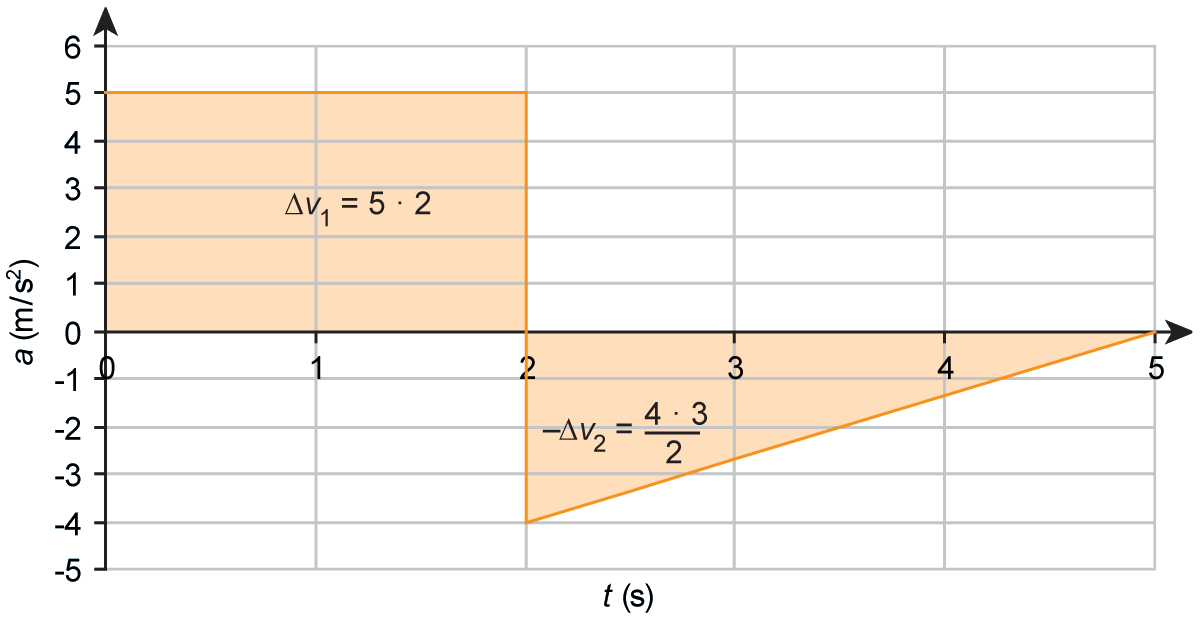
\includegraphics[width=0.8\textwidth]{accelerationTime.png}
        \caption{Acceleration-tid diagram. Källa: \textcite{Fraenkel}}
        \label{fig:acc}
    \end{figure}

Acceleration-tiddiagram (se figur \ref{fig:acc})

\printbibliography

\end{document}
